%============================================================
%  Capitolo 7 – Reti Neurali Convoluzionali (CNN)
%============================================================
\chapter{Reti Neurali Convoluzionali}
\label{ch:cnn}

Le \textbf{Reti Neurali Convoluzionali} (Convolutional Neural Networks, CNN o ConvNet) sono
una classe di architetture progettate specificamente per elaborare dati strutturati su una
griglia, come le immagini (griglia 2D di pixel). La loro idea fondamentale risale ai lavori di
Fukushima sulla gerarchia semplice/complessa della corteccia visiva e alla prima CNN sviluppata
da Yann LeCun a Toronto tra il 1988 e il 1989, successivamente consolidata nel celebre lavoro
su LeNet-5 per il riconoscimento di cifre scritte a mano \citep{bishop2024}.

%------------------------------------------------------------
\section{Limiti delle Reti Completamente Connesse sulle Immagini}
\label{sec:fc-limits}

Nelle reti \emph{fully connected} classiche, ogni neurone riceve in ingresso tutti i valori del
volume di input. Questo approccio \textbf{non scala} alle immagini reali:

\begin{itemize}
  \item Un'immagine CIFAR-10 di dimensioni $32 \times 32 \times 3$ genera già
        $32 \cdot 32 \cdot 3 = 3072$ pesi per un singolo neurone del primo strato nascosto.
  \item Un'immagine di dimensioni più realistiche, ad esempio $200 \times 200 \times 3$,
        porterebbe a $200 \cdot 200 \cdot 3 = 120\,000$ pesi per neurone.
  \item Con molti neuroni i parametri si accumulano rapidamente, determinando
        \textbf{overfitting} e un costo computazionale proibitivo.
\end{itemize}

La connettività totale è dunque uno spreco: pixel vicini sono altamente correlati, e le feature
visive utili (bordi, texture, forme) compaiono in posizioni diverse dell'immagine ma con la
stessa struttura locale.

%------------------------------------------------------------
\section{Volumi 3D e Connettività Locale}
\label{sec:3d-volumes}

\subsection{Organizzazione tridimensionale}
\label{subsec:3d-org}

A differenza di una rete fully connected, i layer di una ConvNet organizzano le proprie unità
in \textbf{tre dimensioni}: larghezza ($W$), altezza ($H$) e profondità ($D$). Il termine
\emph{profondità} qui si riferisce alla terza dimensione del \emph{volume di attivazione} (per
esempio i 3 canali RGB di un'immagine), \emph{non} al numero di layer della rete.

\subsection{Connettività locale}
\label{subsec:local-connectivity}

Per input ad alta dimensionalità è impraticabile collegare ogni unità a tutti i valori del
volume precedente. La soluzione è connettere ogni unità soltanto a una \textbf{regione locale}
dell'input. L'estensione spaziale di questa connessione è un iperparametro chiamato
\textbf{campo recettivo} (receptive field) dell'unità, che coincide con la dimensione del
filtro.

Due proprietà fondamentali:
\begin{enumerate}
  \item \textbf{Connessione locale in 2D}: lungo larghezza e altezza ogni unità vede solo una
        piccola finestra dell'input.
  \item \textbf{Connessione piena in profondità}: lungo la dimensione di profondità la
        connessione si estende all'intera profondità del volume di input (ad esempio tutti e 3
        i canali RGB).
\end{enumerate}

%------------------------------------------------------------
\section{Il Layer di Convoluzione}
\label{sec:conv-layer}

\subsection{Operazione di convoluzione}
\label{subsec:conv-operation}

Il layer convoluzionale fa scorrere (\emph{slide}) un filtro $\mathbf{w}$ di dimensioni
$F \times F \times D$ su tutte le posizioni spaziali del volume di input. In ogni posizione
viene calcolato un \textbf{prodotto scalare} tra il filtro e il corrispondente blocco
dell'input, producendo un singolo scalare di attivazione:

\begin{equation}
  a = \mathbf{w}^{\top} \mathbf{x} + b,
  \label{eq:conv-dot}
\end{equation}

dove $\mathbf{x}$ è il vettore di $F \cdot F \cdot D$ valori del blocco corrente e $b$ è il
bias del filtro. Per un filtro $5 \times 5 \times 3$ il prodotto scalare ha dimensione
$5 \cdot 5 \cdot 3 = 75$.

\begin{figure}[H]
  \centering
  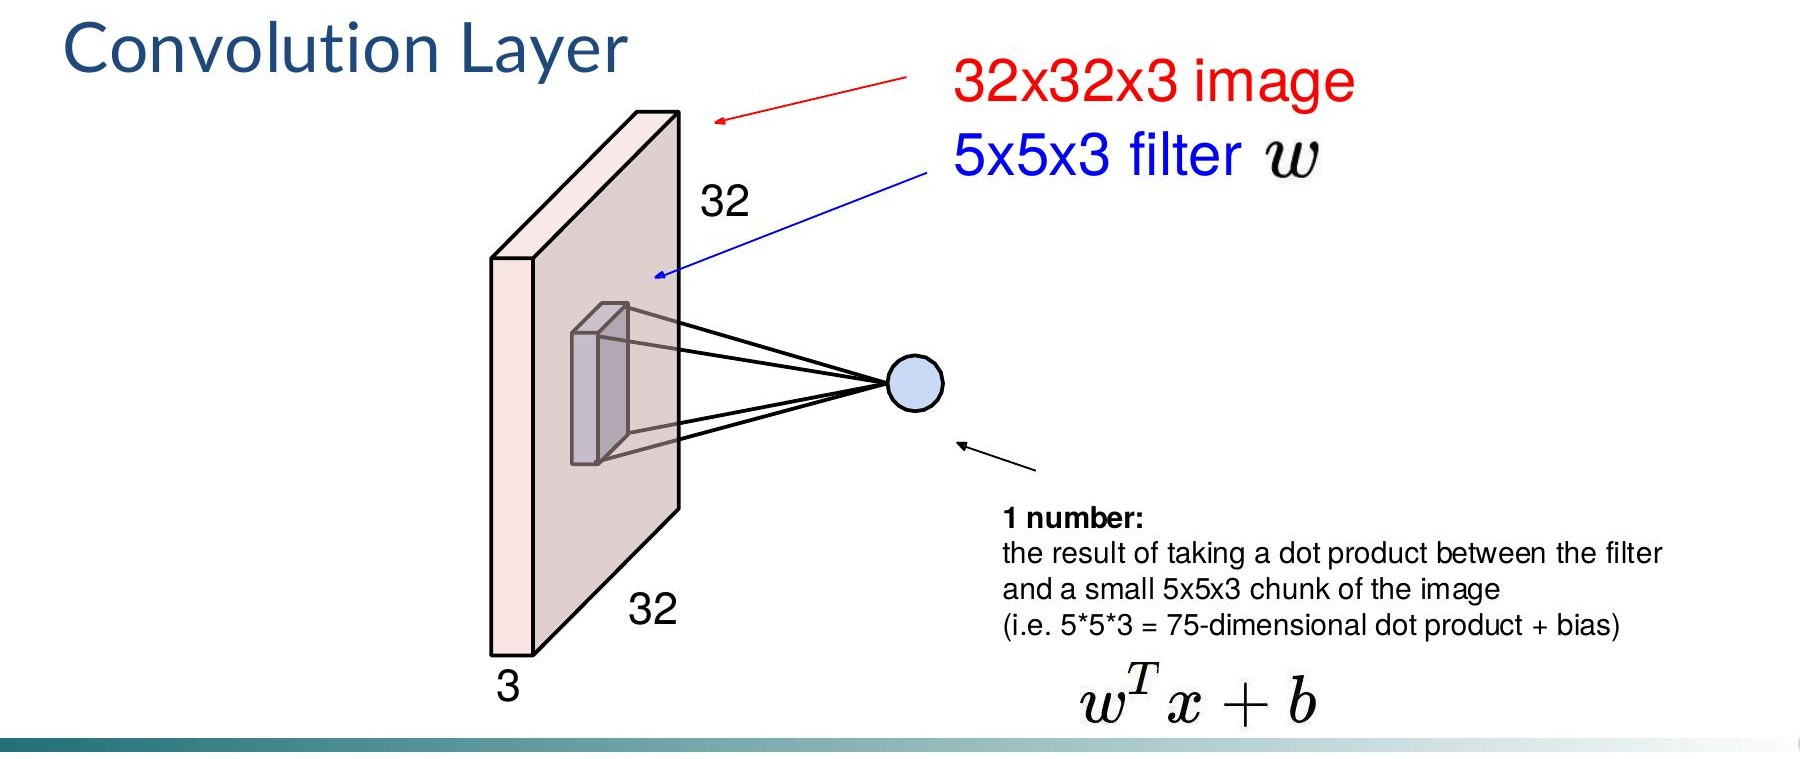
\includegraphics[width=0.82\linewidth]{figures/cf07_conv_dot_product.jpg}
  \caption{Convoluzione di un filtro $5\times5\times3$ su un'immagine $32\times32\times3$:
           ogni neurone di output calcola il prodotto scalare 75-dimensionale
           $\mathbf{w}^{\top}\mathbf{x}+b$ tra il filtro e il blocco locale dell'immagine.}
  \label{fig:conv-dot}
\end{figure}

Il layer si chiama \emph{convoluzionale} perché l'operazione è formalmente legata alla
convoluzione discreta tra due segnali:
\begin{equation}
  (f * g)[x, y] = \sum_{n_1=-\infty}^{+\infty} \sum_{n_2=-\infty}^{+\infty}
    f[n_1, n_2]\cdot g[x - n_1,\, y - n_2],
  \label{eq:conv-formula}
\end{equation}
ovvero una moltiplicazione elemento per elemento e somma tra il filtro e il segnale (immagine).

\subsection{Mappe di attivazione}
\label{subsec:activation-maps}

Facendo scorrere un singolo filtro su tutto il volume di input si ottiene una
\textbf{mappa di attivazione} (activation map) bidimensionale. Se si usano $K$ filtri si
ottengono $K$ mappe, che vengono impilate lungo la dimensione di profondità per formare il
volume di output.

\begin{figure}[H]
  \centering
  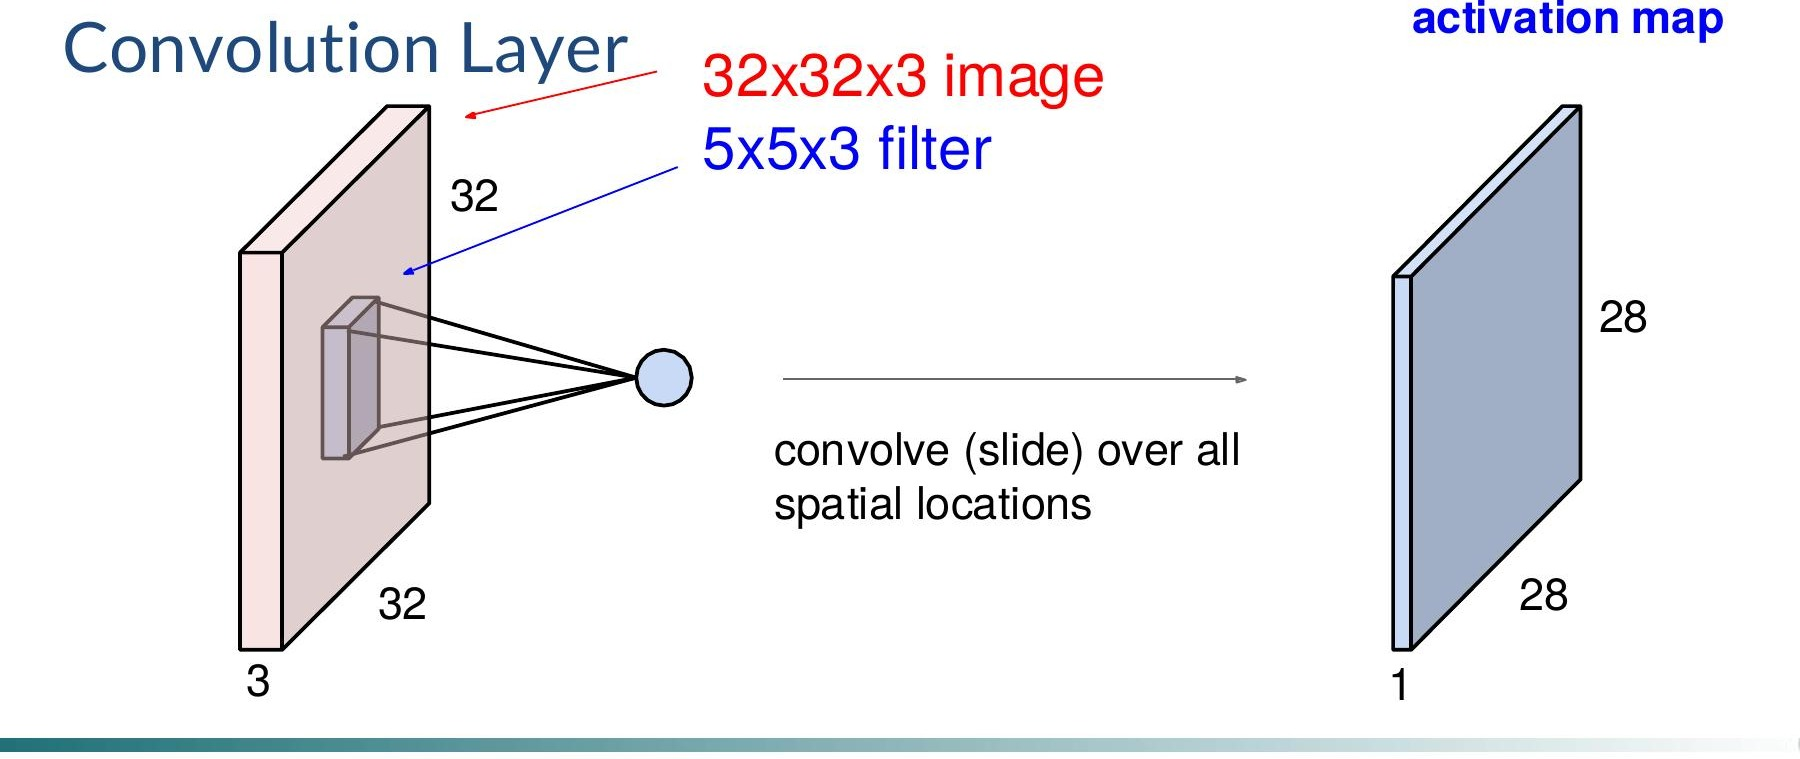
\includegraphics[width=0.82\linewidth]{figures/cf07_activation_map.jpg}
  \caption{Un singolo filtro $5\times5\times3$ applicato sull'immagine $32\times32\times3$
           produce una mappa di attivazione $28\times28\times1$.}
  \label{fig:activation-map}
\end{figure}

\begin{figure}[H]
  \centering
  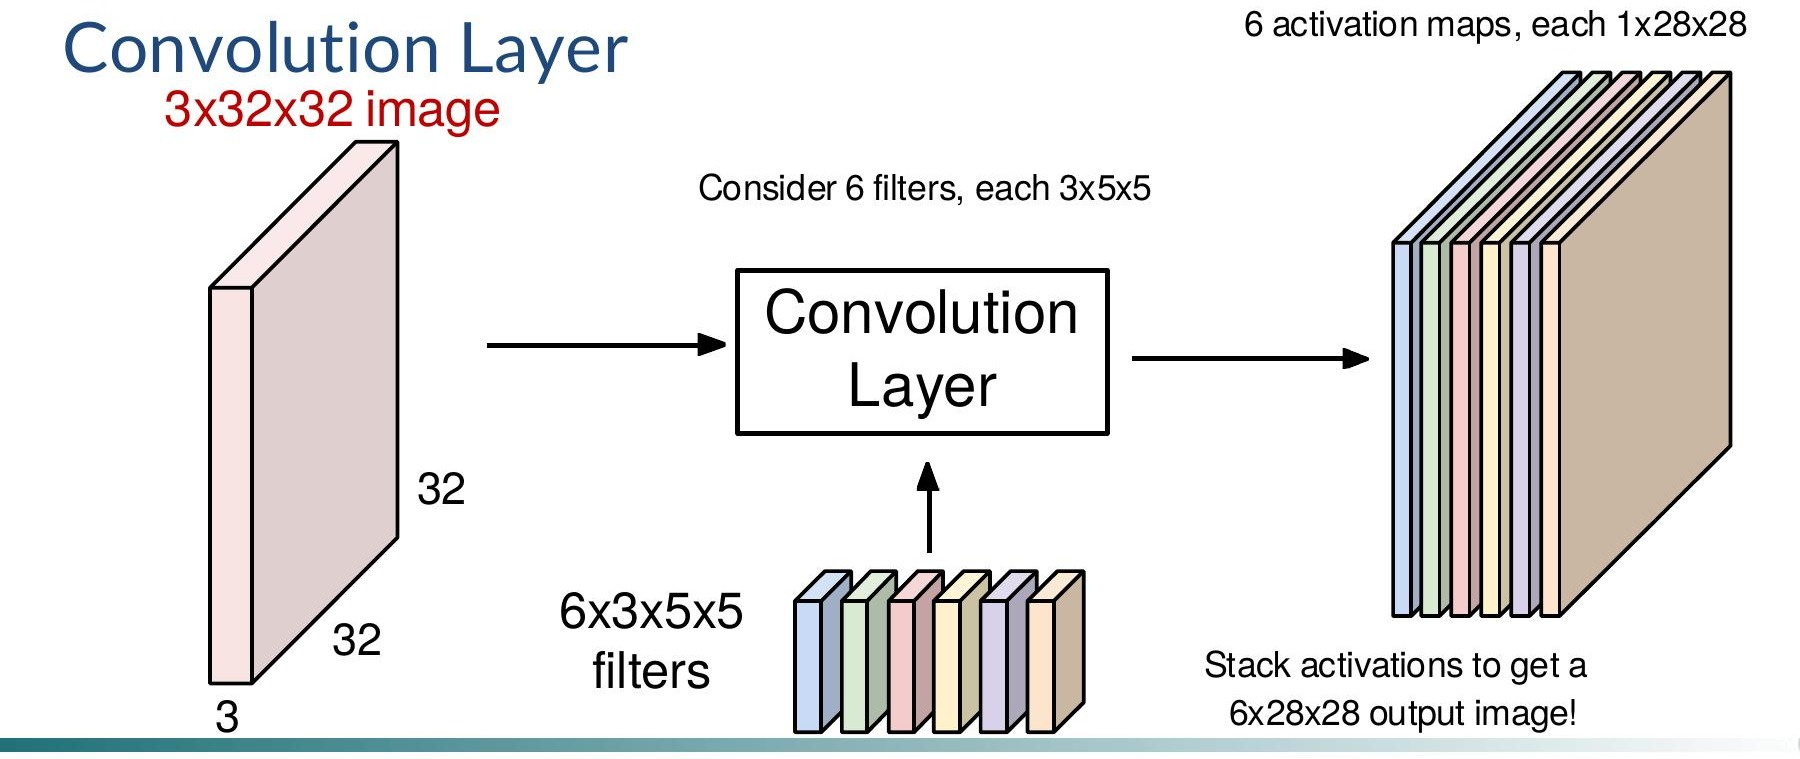
\includegraphics[width=0.90\linewidth]{figures/cf07_six_filters_output.jpg}
  \caption{Con 6 filtri $3\times5\times5$, il layer convoluzionale produce 6 mappe di
           attivazione che vengono impilate per ottenere un output $6\times28\times28$.}
  \label{fig:six-filters}
\end{figure}

\paragraph{Esempio.} Per un'immagine $32 \times 32 \times 3$ con un filtro $5 \times 5 \times
3$ e stride 1, la mappa di attivazione risultante ha dimensioni $28 \times 28 \times 1$. Con
6 filtri si ottiene un volume $28 \times 28 \times 6$.

In generale, con $K$ filtri di dimensione $F \times F \times D_{\text{in}}$:
\begin{itemize}
  \item ogni filtro ha $F \cdot F \cdot D_{\text{in}} + 1$ parametri (incluso il bias);
  \item il volume di output ha profondità $K$;
  \item il numero totale di parametri del layer è $K \cdot (F \cdot F \cdot D_{\text{in}} + 1)$.
\end{itemize}

\subsection{Dimensioni spaziali: stride e zero-padding}
\label{subsec:spatial-dims}

La dimensione spaziale dell'output dipende da tre iperparametri:

\begin{description}
  \item[Stride $S$] Passo con cui il filtro scorre sull'input. Stride maggiore produce output
        più piccoli e sottocampiona la rappresentazione.
  \item[Zero-padding $P$] Aggiunta di zeri intorno al bordo dell'input, che permette di
        controllare la dimensione dell'output.
  \item[Dimensione del filtro $F$] Controlla il campo recettivo locale.
\end{description}

La formula generale per la dimensione spaziale dell'output è:
\begin{equation}
  W_{\text{out}} = \frac{W_{\text{in}} + 2P - F}{S} + 1,
  \label{eq:output-size}
\end{equation}
e analogamente per $H_{\text{out}}$. Se il risultato non è intero, la combinazione
$(F, S, P)$ è incompatibile con l'input dato.

\begin{figure}[H]
  \centering
  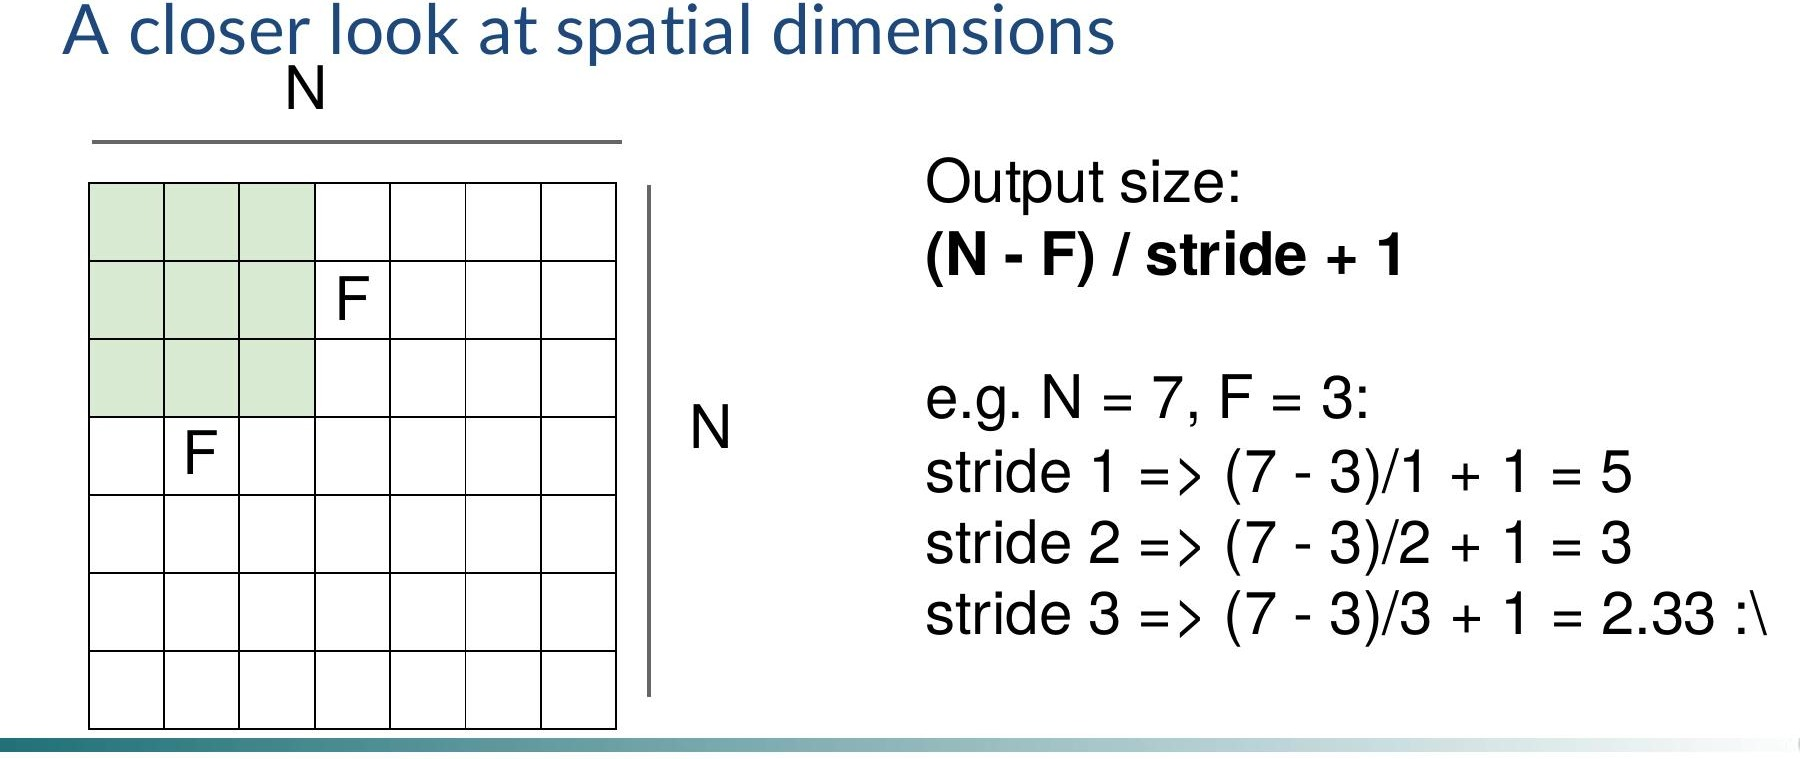
\includegraphics[width=0.82\linewidth]{figures/cf07_stride_formula.jpg}
  \caption{Formula per la dimensione dell'output $(N-F)/\text{stride}+1$ con esempi
           numerici: $N=7,\,F=3$ con stride 1 ($\to5$), stride 2 ($\to3$), stride 3
           (risultato non intero $\Rightarrow$ non valido).}
  \label{fig:stride-formula}
\end{figure}

\paragraph{Zero-padding per preservare la dimensione.} È comune usare stride 1, filtri di
dimensione $F \times F$ e zero-padding pari a $P = (F-1)/2$: questo preserva la dimensione
spaziale dell'input (formula aggiornata: $(N + 2P - F)/S + 1$). Per esempio,
$F = 3 \Rightarrow P = 1$; $F = 5 \Rightarrow P = 2$; $F = 7 \Rightarrow P = 3$.

\begin{figure}[H]
  \centering
  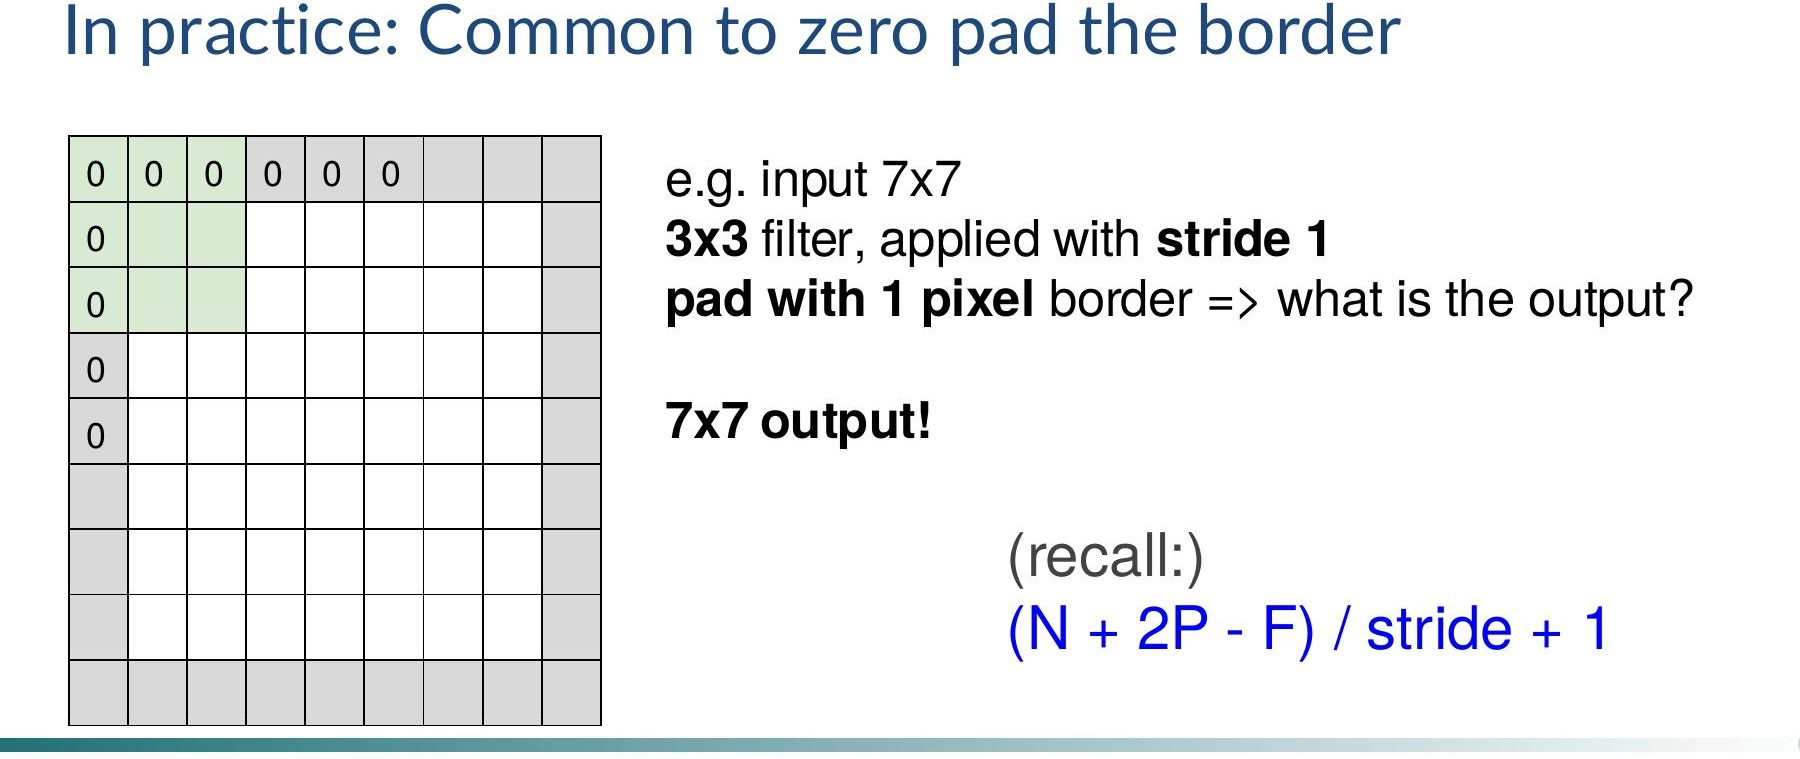
\includegraphics[width=0.82\linewidth]{figures/cf07_zero_padding.jpg}
  \caption{Zero-padding di 1 pixel intorno a un input $7\times7$: con filtro $3\times3$ e
           stride 1, l'output è ancora $7\times7$ (formula: $(7+2\cdot1-3)/1+1=7$).}
  \label{fig:zero-padding}
\end{figure}

\subsection{Convoluzione 1\texttimes1}
\label{subsec:1x1-conv}

Un filtro di dimensione $1 \times 1 \times D_{\text{in}}$ esegue un prodotto scalare
$D_{\text{in}}$-dimensionale in ogni posizione spaziale senza alcuna interazione spaziale.
Questo tipo di convoluzione è utile per:
\begin{itemize}
  \item \textbf{Riduzione di dimensionalità} lungo la profondità (collo di bottiglia),
        senza modificare la risoluzione spaziale.
  \item Aggiungere nonlinearità puntuali tra i layer convoluzionali.
\end{itemize}

%------------------------------------------------------------
\section{Campi Recettivi}
\label{sec:receptive-fields}

Il \textbf{campo recettivo} di un'unità è la regione dell'input originale che influenza il suo
valore di attivazione. Con un kernel di dimensione $K$, ogni elemento dell'output dipende da
una regione $K \times K$ del layer precedente. Ogni convoluzione successiva aggiunge $K-1$
alla dimensione del campo recettivo; con $L$ layer:

\begin{equation}
  \text{RF} = 1 + L \cdot (K - 1).
  \label{eq:receptive-field}
\end{equation}

\begin{figure}[H]
  \centering
  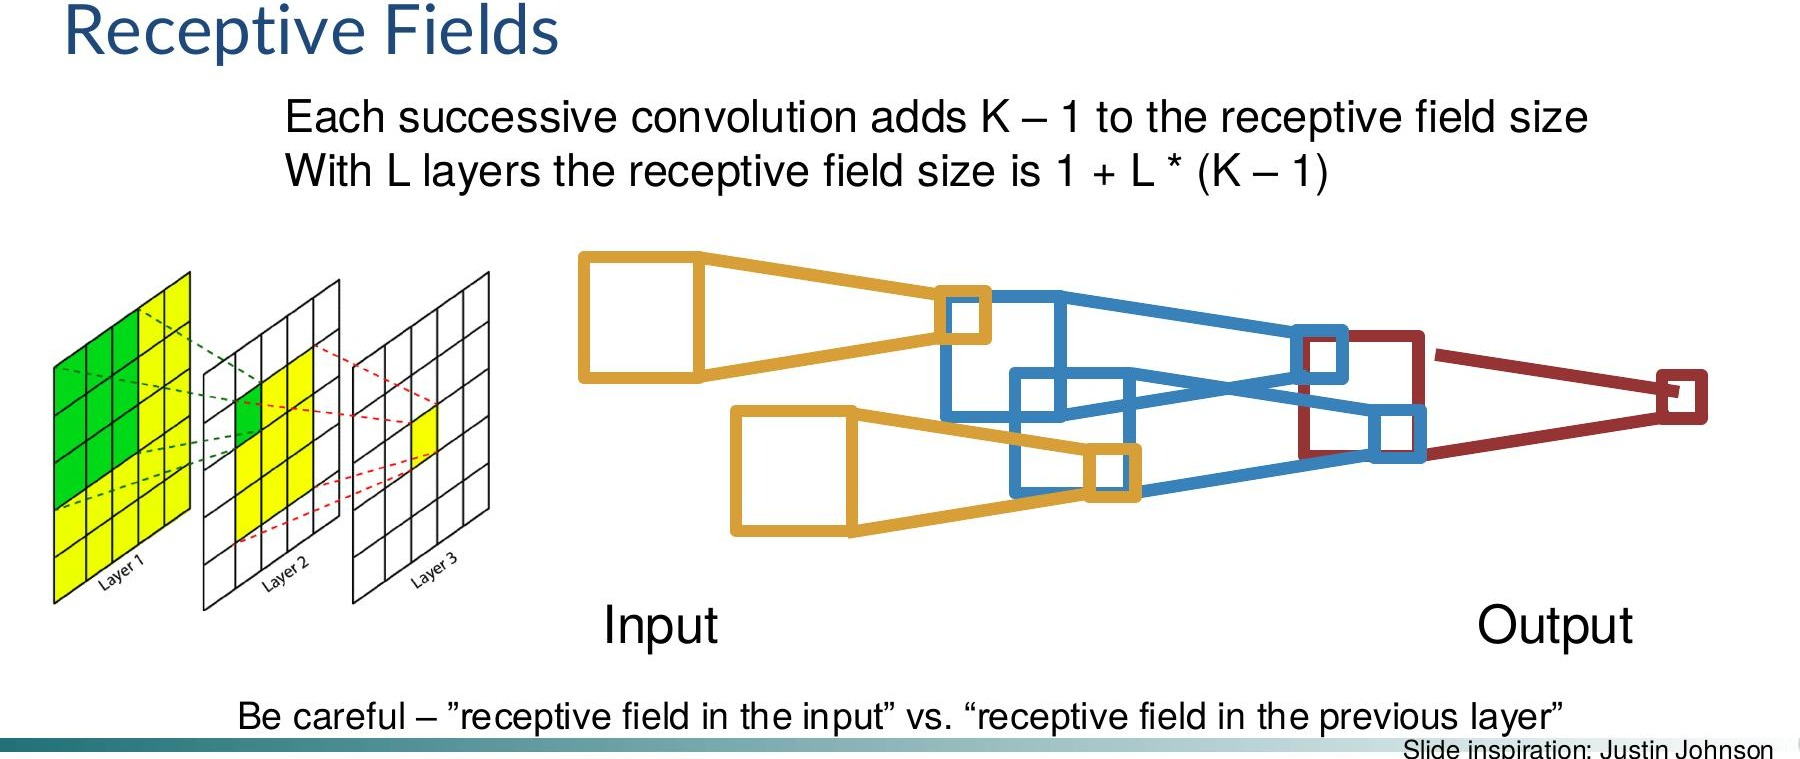
\includegraphics[width=0.88\linewidth]{figures/cf07_receptive_fields.jpg}
  \caption{Campi recettivi attraverso tre layer convoluzionali successivi: ogni layer
           espande la porzione dell'input originale vista da ciascuna unità. Con $L$ layer
           e kernel $K$, il campo recettivo totale sull'input è $1+L(K-1)$.
           Nota: ``receptive field in the input'' vs.\  ``receptive field in the previous
           layer'' sono concetti distinti.}
  \label{fig:receptive-fields}
\end{figure}

\paragraph{Problema per immagini grandi.}
Per immagini grandi è necessario un numero molto elevato di layer affinché ogni unità
dell'output ``veda'' l'intera immagine. La \textbf{soluzione} è il sottocampionamento
(\emph{downsampling}) all'interno della rete, ottenuto con:
\begin{itemize}
  \item \textbf{Convoluzione con stride $> 1$}: riduce direttamente la risoluzione spaziale.
  \item \textbf{Pooling}: layer dedicati al sottocampionamento (vedi
        Sezione~\ref{sec:pooling}).
\end{itemize}

%------------------------------------------------------------
\section{Cosa Imparano i Filtri Convoluzionali?}
\label{sec:what-filters-learn}

I filtri del primo layer fungono da \emph{template} locali sull'immagine. Dopo l'addestramento
su grandi dataset, i filtri del primo layer imparano a rilevare feature di basso livello come
bordi orientati in varie direzioni, colori opposti e frequenze spaziali diverse (in AlexNet,
64 filtri $3\times11\times11$). Nei layer successivi le mappe combinano le risposte precedenti,
rilevando pattern di complessità crescente: angoli al secondo layer, parti di oggetti al
terzo, interi oggetti agli strati più profondi.

%------------------------------------------------------------
\section{Il Layer di Pooling}
\label{sec:pooling}

Il layer di pooling serve a \textbf{ridurre la risoluzione spaziale} delle mappe di
attivazione, rendendo la rappresentazione più compatta e introducendo una certa
\textbf{invarianza traslazionale}. Opera in modo \emph{indipendente} su ciascuna mappa.

\subsection{Max Pooling}
\label{subsec:max-pooling}

Il \textbf{Max Pooling} è la variante più comune: data una finestra di dimensioni
$P_H \times P_W$ con stride $S$, si prende il massimo dei valori nella finestra.

\begin{figure}[H]
  \centering
  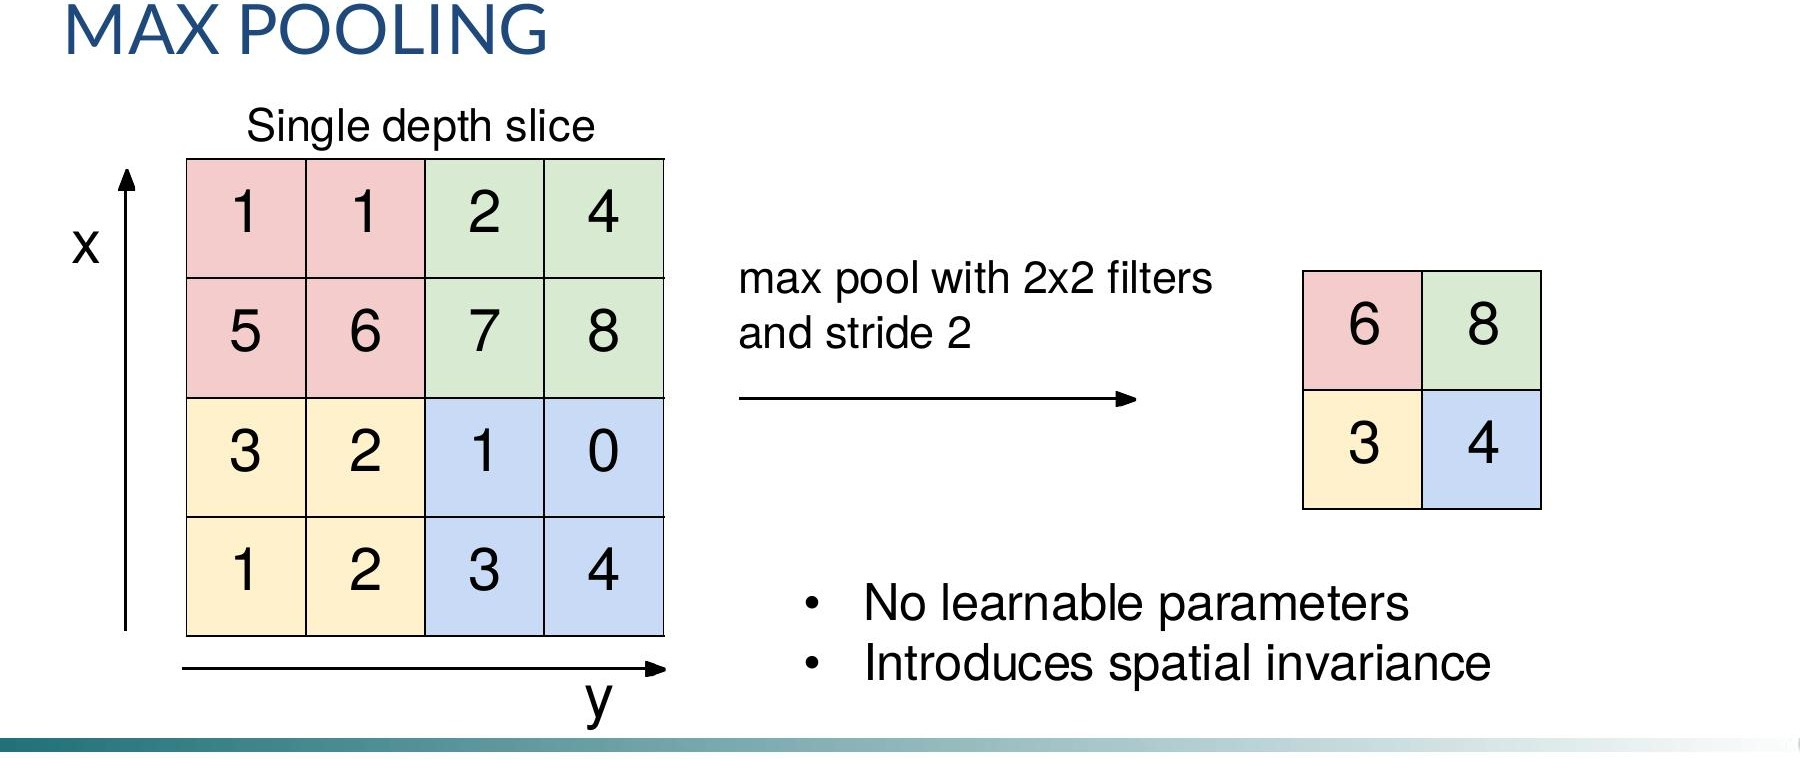
\includegraphics[width=0.82\linewidth]{figures/cf07_max_pooling.jpg}
  \caption{Max pooling $2\times2$ con stride 2 su una singola mappa $4\times4$: ogni
           quadrante $2\times2$ viene sostituito dal suo valore massimo, dimezzando la
           risoluzione spaziale. Nessun parametro apprendibile; introduce invarianza
           spaziale locale.}
  \label{fig:max-pooling}
\end{figure}

In formule, il max pooling $2\times2$ con stride 2 sull'esempio delle slide produce:
\begin{equation}
  \begin{pmatrix}
    1 & 1 & 2 & 4 \\
    5 & 6 & 7 & 8 \\
    3 & 2 & 1 & 0 \\
    1 & 2 & 3 & 4
  \end{pmatrix}
  \xrightarrow{\text{MaxPool }2\times2,\,s=2}
  \begin{pmatrix}
    6 & 8 \\
    3 & 4
  \end{pmatrix}.
  \label{eq:maxpool-example}
\end{equation}

Proprietà chiave: nessun parametro apprendibile; invarianza spaziale locale (piccole
traslazioni non cambiano l'output); riduzione spaziale tipicamente di un fattore 2.

\subsection{Altre varianti di pooling}
\label{subsec:other-pooling}

\begin{description}
  \item[Average Pooling] Calcola la media dei valori nella finestra.
  \item[Global Average Pooling (GAP)] Riduce ogni mappa a un unico scalare (media globale).
        Usato in GoogLeNet e ResNet come alternativa ai layer FC finali.
  \item[LP-Norm Pooling] $\bigl(\sum_i x_i^p\bigr)^{1/p}$; per $p\to\infty$ si ottiene il
        max pooling.
\end{description}

%------------------------------------------------------------
\section{Il Layer Fully Connected}
\label{sec:fc-layer}

Dopo un certo numero di layer CONV/ReLU/POOL, le mappe di attivazione vengono
\textbf{appiattite} (\emph{flatten}) in un vettore unidimensionale e passate a uno o più
\textbf{layer fully connected} (FC), dove ogni neurone è connesso a tutti i valori
dell'input. Questi layer eseguono la classificazione vera e propria combinando le feature
estratte dai layer convoluzionali. Il layer finale produce un punteggio per ciascuna delle
$C$ classi, tipicamente seguito da \textbf{softmax} per ottenere una distribuzione di
probabilità.

%------------------------------------------------------------
\section{Architettura Tipica di una ConvNet}
\label{sec:typical-arch}

Una ConvNet classica è costruita impilando ripetutamente layer CONV$+$ReLU, seguiti
periodicamente da layer di pooling e, alla fine, da layer FC:

\begin{equation}
  \underbrace{[(\text{CONV} \to \text{ReLU})^{\times N} \to \text{POOL?}]^{\times M}}
    _{\text{estrazione di feature}}
  \;\longrightarrow\;
  \underbrace{(\text{FC} \to \text{ReLU})^{\times K} \to \text{Softmax}}
    _{\text{classificazione}}
  \label{eq:typical-arch}
\end{equation}

dove tipicamente $N \lesssim 5$, $M$ è grande, $0 \le K \le 2$.

\paragraph{Trend moderni.}
\begin{itemize}
  \item Filtri piccoli ($3 \times 3$) in stack profondi al posto di filtri grandi (due
        $3\times3$ hanno lo stesso campo recettivo di un $5\times5$ ma con meno parametri e
        più nonlinearità).
  \item Eliminazione progressiva del pooling, sostituito da convoluzioni con stride 2.
  \item Architetture come \textbf{ResNet} e \textbf{GoogLeNet} sfidano il paradigma
        sequenziale con connessioni residue e moduli Inception.
\end{itemize}

\subsection{Esempio di stack convoluzionale}
\label{subsec:conv-stack-example}

\begin{table}[H]
  \centering
  \caption{Evoluzione delle dimensioni dei volumi in una ConvNet di esempio su
           un'immagine $32\times32\times3$.}
  \label{tab:conv-stack}
  \small
  \begin{tabular}{lccc}
    \toprule
    \textbf{Layer} & \textbf{Filtri / Operazione} & \textbf{Output} & \textbf{Param.} \\
    \midrule
    Input          & --                                       & $32\times32\times3$  & 0 \\
    CONV1+ReLU     & 6 filtri $5\times5$, $s=1$, $P=0$       & $28\times28\times6$  & 456 \\
    CONV2+ReLU     & 10 filtri $5\times5$, $s=1$, $P=0$      & $24\times24\times10$ & 1510 \\
    MaxPool        & $2\times2$, $s=2$                        & $12\times12\times10$ & 0 \\
    FC+ReLU        & 120 unità                                & $120$                & 173\,640 \\
    Softmax        & 10 classi                                & $10$                 & 1210 \\
    \bottomrule
  \end{tabular}
\end{table}

%------------------------------------------------------------
\section{Proprietà Fondamentali delle ConvNet}
\label{sec:cnn-properties}

\subsection{Parameter sharing}
\label{subsec:param-sharing}

In un layer convoluzionale, lo \textbf{stesso filtro} (con gli stessi pesi) viene applicato
in \emph{tutte} le posizioni spaziali dell'input. Questo si basa sull'assunzione che una
feature utile in una posizione sia utile anche in un'altra (\emph{equivarianza
traslazionale}). Il vantaggio pratico è una drastica riduzione del numero di parametri.

\subsection{Equivarianza traslazionale}
\label{subsec:equivariance}

La convoluzione è \textbf{equivariante per traslazione}: traslare l'input causa una
traslazione corrispondente nella mappa di attivazione. Formalmente, se $T_\Delta$ è una
traslazione di $\Delta$ posizioni:
\begin{equation}
  f(T_\Delta(\mathbf{x})) = T_\Delta(f(\mathbf{x})).
  \label{eq:equivariance}
\end{equation}
Il pooling con stride $> 1$ introduce invece \textbf{invarianza approssimata}: una
traslazione di 1 pixel nell'input diventa 0.5 pixel dopo un pooling $2\times2$.

\subsection{Connessioni sparse}
\label{subsec:sparse-conn}

Ogni unità dell'output dipende solo da una piccola regione locale dell'input invece che da
tutti i pixel, riducendo la complessità computazionale e favorendo la generalizzazione.

%------------------------------------------------------------
\section{Riepilogo dei Componenti Principali}
\label{sec:cnn-summary}

\begin{table}[H]
  \centering
  \caption{Riepilogo dei layer fondamentali di una ConvNet.}
  \label{tab:cnn-summary}
  \small
  \begin{tabular}{p{2.8cm}p{5.2cm}p{4.2cm}}
    \toprule
    \textbf{Layer} & \textbf{Funzione} & \textbf{Iperparametri principali} \\
    \midrule
    CONV            & Estrazione di feature locali tramite
                      prodotti scalari con filtri appresi &
                      $F$, $K$, $S$, $P$ \\
    \addlinespace
    ReLU            & Nonlinearità puntuale $\max(0,x)$ & -- \\
    \addlinespace
    POOL (Max/Avg)  & Sottocampionamento spaziale &
                      Finestra $P_H\times P_W$, $S$ \\
    \addlinespace
    FC              & Classificazione globale & Numero di unità \\
    \addlinespace
    Softmax         & Distribuzione di probabilità sulle classi & -- \\
    \bottomrule
  \end{tabular}
\end{table}

\paragraph{Regole pratiche.}
\begin{enumerate}
  \item Preferire filtri piccoli ($3 \times 3$) in stack profondi.
  \item Usare zero-padding $P = (F-1)/2$ per preservare la risoluzione nei layer CONV con
        stride 1.
  \item Il pooling $2 \times 2$ con stride 2 è la scelta più comune; il global average
        pooling è preferibile nei classificatori moderni.
  \item Verificare sempre che l'equazione~\eqref{eq:output-size} dia un intero.
  \item Aumentare la profondità (più filtri per layer) man mano che la risoluzione spaziale
        diminuisce, per mantenere la capacità rappresentativa della rete.
\end{enumerate}

Come sottolinea \citet{bishop2024}, la scelta dell'architettura convoluzionale è guidata da
considerazioni sul campo recettivo, dalla capacità del modello rispetto alla dimensione del
dataset e dal costo computazionale del training e dell'inference.
